\chapter{离散数学}
\section{图论}

\noindent 警察抓强盗的问题 (Cops and Robber Problem)

有一个图, 警察位于一个节点上, 强盗可以选择初始节点, 之后警察和强盗轮流在图上移动, 可以从一个节点走到邻接的节点, 也可以原地不动. 如果警察一定能抓到强盗, 则称这个图是警察必胜的, 反之称为强盗必胜的. 给定一个图, 判断是警察必胜还是强盗必胜.

~

定义一类节点为陷阱点如下: 

如果一个节点 $ P $ 与一个节点 $ A $ 邻接, 且 $ P $ 的其他所有邻居都和 $ A $ 邻接, 则称 $ P $ 是一个陷阱节点 ( Pitfall ), 含义是只要强盗在 $ P $ 点而警察在 $ A $ 点时, 警察就获胜了. 这里 $ A $ 点称为攻击点 ( Attack ).

引理: 如果图中存在一个陷阱节点, 则可以去掉这个节点和它关联的边, 不影响警察和强盗的输赢.

\begin{figure*}[htbp]
\centering
 \begin{tabular}{c @{\hspace{.2\textwidth}} c}
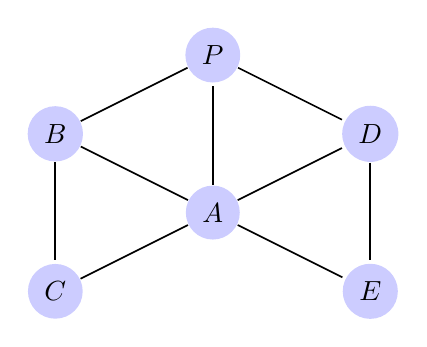
\begin{tikzpicture}[> = stealth,shorten > = 1pt,auto,	node distance = 3cm,semithick ,auto=left,every node/.style={circle,fill=blue!20}]
	\node (n1) at (-2,1.)		{$B$};
	\node (n2) at (-2,-1.)  	{$C$};
	\node (n3) at (2,1.) 	{$D$};
	\node (n4) at (2,-1) 	{$E$};
	\node (n5) at (0,0) 	{$A$};
	\node (n6) at (0,2)	{$P$};
	\draw (n1)--(n2);
	\draw (n3)--(n4);
	\draw (n1)--(n5) -- (n4);
	\draw (n2)--(n5) -- (n3);
	\draw (n1)--(n6) -- (n3);
	\draw (n5)--(n6);

	%\draw [red,very thick](n4)--(n5);
	%\draw [red,very thick] (n1) .. controls (-2,-2.5)  ..(n4);
	%\draw [red,very thick](n1) .. controls (2,-3.5) 	..(n5);
\end{tikzpicture} & 
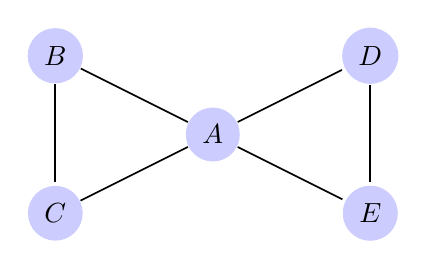
\begin{tikzpicture}[> = stealth,shorten > = 1pt,auto,	node distance = 3cm,semithick,auto=left,every node/.style={circle,fill=blue!20}]
	\node (n1) at (-2,1.)		{$B$};
	\node (n2) at (-2,-1.)  	{$C$};
	\node (n3) at (2,1.) 	{$D$};
	\node (n4) at (2,-1) 	{$E$};
	\node (n5) at (0,0) 	{$A$};
	\draw (n1)--(n2);
	\draw (n3)--(n4);
	\draw (n1)--(n5) -- (n4);
	\draw (n2)--(n5) -- (n3);
\end{tikzpicture}
 \\
$ G $ & $ H $
\end{tabular}

\end{figure*}

证明: 假设原图是 $ G $, 有一个陷阱节点 $ P $ 和攻击点 $ A $, 移除陷阱节点 $ P $ 和其相连的边之后得到的图为 $ H $. 如果 $ H $ 是警察必胜的, 则在 $ G $ 中警察也必胜, 原因是在 $ G $ 中警察可以复制 $ H $ 中的策略, 当强盗位于 $ P $ 点时, 注意到无论下一步强盗走到哪个节点, 或者不动, 都可以在 $ A $ 点一步到达, 对于警察来说, 强盗位于 $ P $ 点就像位于 $ A $ 点一样, 所以警察沿用原来的策略以 $ A $ 点为目标即可. 反过来如果强盗在 $ G $ 中必胜, 则他在 $ H $ 中也必胜. 

另一方面, 如果强盗在 $ H $ 中必胜, 也是同样的道理, 在 $ G $ 中, 当警察位于点 $ P $ 时, 强盗可以当做警察在
$ A $ 点一样按原来的策略逃脱. 这一条的对偶命题同样成立: 如果警察在 $ G $ 中必胜, 则在 $ H $ 中也必胜.

以上证明了一个图去掉一个陷阱节点后与原图是等价的. 这样可以不断去掉陷阱节点, 直到不能去掉为止. 如果最终剩余一个节点, 则警察必胜. 否则强盗必胜.

\newpage
%------------------------------------------------------------------------------%
\noindent 环球城市数学竞赛 1982 年初中组春季赛

某国城市数量多于 101 个, 这个国家的首都与其他 100 个城市有直达航班, 而首都之外的城市都与其他 10 个城市有(包括首都在内)直达航班, 并且从这个国家的任一城市可乘飞机达到任一另外的城市(不一定是直达, 中途可能转机). 

求证: 可以关闭与首都相连的一半直达航班, 使得仍然可以从这个国家的任一城市乘飞机到达任一另外的城市.

~

证明: 构造一个图 $G$, 一个节点表示一个城市, 若两城市有直达航班, 则对应两个节点之间连一条边. 记首都对应的节点为 $M$. 再构造图 $G'$, 它是在 $G$ 的基础上去掉了 $M$ 节点以及跟 $M$ 相连的边. 由题意描述, $G$ 是一个连通图, $G'$ 不一定连通, 可能有多个连通分量, 且 $G'$ 的每个连通分量至少有一个顶点在 $G$ 中与 $M$ 点相连. 在 $G$ 中除了 $M$ 外每个点的度数为 10, 则与 $M$ 相连的那些点在 $G'$ 中度数为 9, 与 $M$ 不相连的点在 $G'$ 中的度数仍为 10. 而任意图中, 所有顶点的度数之和为偶数, 所以 $G'$ 中每个连通分量的顶点度数之和也要是偶数, 说明每个联通分量至少有两个度数为 9 的点, 进一步可知每个联通分量至少有两个顶点在 $G$ 中与 $M$ 相连. 而 $G$ 中 $M$ 的度数为 100, 于是 $G'$ 中的连通分量最多有 50 个, 这样只要保留 $M$ 到 $G'$ 中的每个连通分量有一条边, 其他 $M$ 关联的边删掉, 则得到的图仍然是连通的.
\begin{figure*}[htbp]
\centering
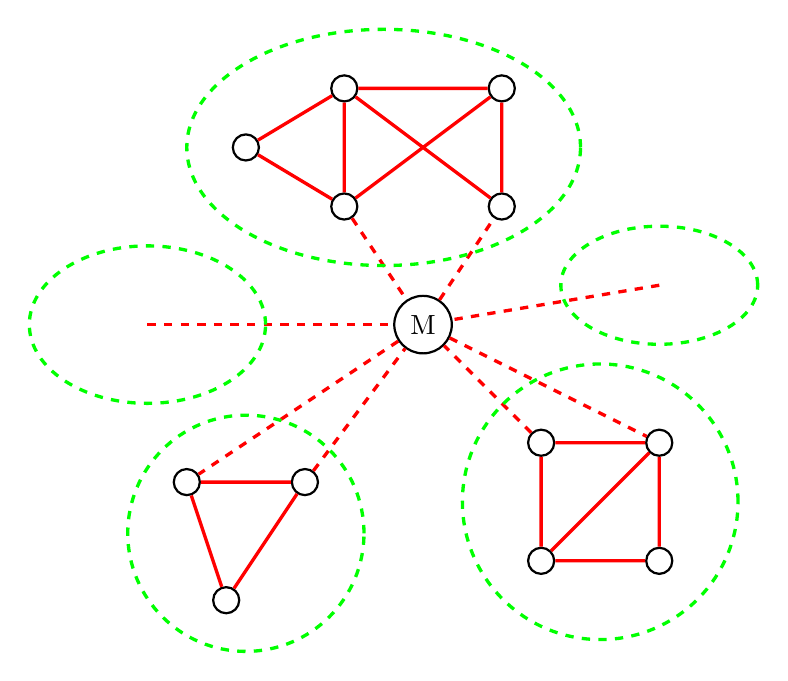
\begin{tikzpicture}[scale=0.5]
\begin{scope}[every node/.style={circle,thick,draw}]
    \node (A) at (-5,-5) {};
    \node (B) at (-6,-2) {};
    \node (C) at (-3,-2) {};
    \node (M) at (0,2) {M};
    \node (D) at (6,-1) {};
    \node (E) at (6,-4) {};
    \node (F) at (3,-4) {};
    \node (G) at (3,-1) {};
    \node (H) at (-4.5,6.5) {};
    \node (I) at (2,8) {};
    \node (J) at (2,5) {};
    \node (K) at (-2,5) {};
    \node (L) at (-2,8) {};
\end{scope}
\begin{scope}[]
\draw[very thick,red] (A) -- (B) -- (C) -- (A);
\draw[very thick,red,dashed] (C) -- (M) -- (B);
\draw[very thick,red] (D) -- (E) -- (F) -- (G) -- (D) -- (F);
\draw[very thick,red,dashed] (G) -- (M) -- (D);
\draw[very thick,red] (I) -- (L) -- (K) -- (I) -- (J) -- (L) -- (H) -- (K);
\draw[very thick,red,dashed] (K) -- (M) -- (J);
\draw[very thick,red,dashed] (-7,2) -- (M);
\draw[very thick,red,dashed] (6,3) -- (M);
\end{scope}
\draw[very thick,green,dashed] (-4.5,-3.3) circle (3cm);
\draw[very thick,green,dashed] (4.5,-2.5) circle (3.5cm);
\draw[very thick,green,dashed] (-1,6.5) ellipse (5cm and 3cm);
\draw[very thick,green,dashed] (6,3) ellipse (2.5cm and 1.5cm);
\draw[very thick,green,dashed] (-7,2) ellipse (3cm and 2cm);
\end{tikzpicture}
\end{figure*}

\newpage
%------------------------------------------------------------------------------%









